% Sketch output, version 0.3 (build 2d, Wed Apr 20 23:38:45 2011)
% Output language: PGF/TikZ,LaTeX
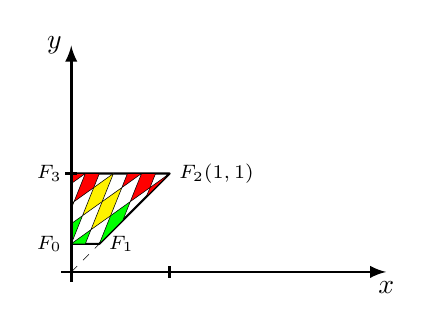
\begin{tikzpicture}[line join=round,line width=0.2pt,>=latex]
\filldraw[fill=none,line width=0.75pt](7,.357)--(7.357,.357)--(8.25,1.25)--(7,1.25)--cycle;
\draw[dashed](7,0)--(7.357,.357);
\filldraw[fill=red](7.952,.952)--(8.25,1.25)--(8,1.071)--cycle;
\filldraw[fill=red](7.75,.893)--(8,1.071)--(8.071,1.25)--(7.893,1.25)--cycle;
\filldraw[fill=red](7.714,1.25)--(7.643,1.071)--(7.893,1.25)--cycle;
\filldraw[fill=red](7.179,1.25)--(7.036,.893)--(7.286,1.071)--(7.357,1.25)--cycle;
\filldraw[fill=red](7,1.25)--(7,1.122)--(7.179,1.25)--cycle;
\filldraw[fill=yellow](7.25,.536)--(7.5,.714)--(7.643,1.071)--(7.393,.893)--cycle;
\filldraw[fill=yellow](7.286,1.071)--(7.143,.714)--(7.393,.893)--(7.536,1.25)--cycle;
\filldraw[fill=yellow](7.036,.893)--(7,.804)--(7,.867)--cycle;
\filldraw[fill=green](7.357,.357)--(7.655,.655)--(7.75,.893)--(7.5,.714)--cycle;
\filldraw[fill=green](7,.357)--(7.179,.357)--(7.25,.536)--cycle;
\filldraw[fill=green](7,.357)--(7.143,.714)--(7,.612)--cycle;
\draw[line width=1pt](7.075,1.25)--(6.925,1.25);
\draw[line width=1pt](8.25,.075)--(8.25,-.075);
\draw[->,line width=1pt](7,-.125)--(7,2.875);
\draw[->,line width=1pt](6.875,0)--(11,0);

    \coordinate [label=below:$x$] (X) at (11,0);
    \coordinate [label=left:$y$] (Y) at (7,2.875);
  
    \coordinate [label=180:\scriptsize$F_0$] (p0F) at (7,.357);
    \coordinate [label=000:\scriptsize$F_1$] (p1F) at (7.357,.357);
    \coordinate [label=000:{\scriptsize$F_2(1,1)$}] (p2F) at (8.25,1.25);
    \coordinate [label=180:\scriptsize$F_3$] (p3F) at (7,1.25);
  \end{tikzpicture}% End sketch output
